% ============================================================================
% CHAPTER 4: SYSTEM IMPLEMENTATION
% ============================================================================

\chapter{SYSTEM IMPLEMENTATION}

\section{MODULE IMPLEMENTATION}

This section describes the implementation of key system modules with relevant code excerpts and explanations, providing sufficient detail for reproducibility while focusing on the most architecturally significant components.

\subsection{Development Environment}

The system is implemented in Python using modern deep learning frameworks and specialized libraries for EEG processing. Table \ref{tab:packages} lists the primary packages and their purposes. PyTorch serves as the core deep learning framework, providing automatic differentiation, GPU acceleration, and a rich ecosystem of model building blocks. PyTorch Geometric extends PyTorch with efficient implementations of graph neural network operations, including the Graph Attention layers used in the GNN branch. MNE-Python handles EEG-specific data loading and preprocessing, providing robust implementations of filtering, artifact rejection, and epoch extraction that follow established best practices in the neuroimaging community.

\begin{table}[H]
    \centering
    \small
    \caption{Primary Python Packages and Versions}
    \label{tab:packages}
    \begin{tabularx}{\textwidth}{|L{3.5cm}|L{2cm}|X|}
        \hline
        \textbf{Package} & \textbf{Version} & \textbf{Purpose} \\
        \hline
        Python & 3.10+ & Programming language \\
        \hline
        PyTorch & 2.0+ & Deep learning framework \\
        \hline
        PyTorch Geometric & 2.3+ & Graph neural network operations \\
        \hline
        MNE-Python & 1.5+ & EEG data loading and preprocessing \\
        \hline
        PyWavelets & 1.4+ & Wavelet transforms (WPD, CWT) \\
        \hline
        NumPy & 1.24+ & Numerical computing \\
        \hline
        SciPy & 1.10+ & Signal processing utilities \\
        \hline
        scikit-learn & 1.3+ & Metrics and utilities \\
        \hline
        Captum & 0.6+ & Model interpretability (IG, LRP) \\
        \hline
        Matplotlib & 3.7+ & Visualization \\
        \hline
        tqdm & 4.65+ & Progress bars \\
        \hline
    \end{tabularx}
\end{table}

\subsection{Transformer Encoder Implementation}

The Transformer encoder processes CWT scalograms using patch-based tokenization followed by self-attention, adapting the Vision Transformer architecture for time-frequency analysis of EEG signals. The implementation begins with a patch embedding layer that divides the input scalogram into a grid of non-overlapping patches and projects each patch to the model dimension. A learnable classification token and positional encodings are added before the sequence passes through multiple Transformer encoder layers.

\begin{lstlisting}[language=Python, caption={Transformer Encoder Core Structure (transformer\_encoder.py)}]
class EEGTransformerEncoder(nn.Module):
    def __init__(self, img_size=(64, 128), patch_size=(8, 16),
                 d_model=128, nhead=4, num_layers=4):
        super().__init__()

        # Patch embedding: convert scalogram to token sequence
        self.patch_embed = PatchEmbedding(
            img_size=img_size, patch_size=patch_size,
            in_channels=1, embed_dim=d_model
        )

        # Learnable CLS token for classification
        self.cls_token = nn.Parameter(torch.randn(1, 1, d_model) * 0.02)

        # Positional encoding (learnable)
        n_patches = self.patch_embed.n_patches + 1  # +1 for CLS
        self.pos_encoding = nn.Parameter(
            torch.randn(1, n_patches, d_model) * 0.02
        )

        # Transformer encoder layers
        encoder_layer = nn.TransformerEncoderLayer(
            d_model=d_model, nhead=nhead, dim_feedforward=512,
            dropout=0.1, activation='gelu', batch_first=True
        )
        self.transformer = nn.TransformerEncoder(
            encoder_layer, num_layers=num_layers
        )

    def forward(self, x):
        # x: (B, 1, 64, 128) - scalogram
        B = x.shape[0]

        # Patch embedding: (B, 64, 128)
        x = self.patch_embed(x)

        # Prepend CLS token
        cls = self.cls_token.expand(B, -1, -1)
        x = torch.cat([cls, x], dim=1)

        # Add positional encoding
        x = x + self.pos_encoding

        # Transformer forward
        x = self.transformer(x)

        # Return CLS token output
        return x[:, 0]  # (B, 128)
\end{lstlisting}

The implementation leverages PyTorch's built-in TransformerEncoderLayer, which encapsulates multi-head self-attention followed by a position-wise feed-forward network with layer normalization and residual connections. The patch embedding layer is implemented as a convolutional layer with kernel size and stride equal to the patch size, efficiently extracting and projecting all patches in a single operation. The CLS token and positional encodings are initialized with small random values (scaled by 0.02) following best practices from the Vision Transformer literature.

\subsection{Graph Attention Network Implementation}

The GNN branch models electrode spatial relationships using multi-head attention over the electrode graph, learning which connections between electrodes are most informative for depression detection. The implementation uses the GATConv layer from PyTorch Geometric, which implements the Graph Attention mechanism with efficient sparse matrix operations.

\begin{lstlisting}[language=Python, caption={GNN Encoder Core Structure (gnn\_encoder.py)}]
class EEGGraphAttentionNetwork(nn.Module):
    def __init__(self, in_features=576, hidden_dim=256,
                 out_dim=128, num_heads=4):
        super().__init__()

        # Input projection
        self.input_proj = nn.Linear(in_features, hidden_dim)

        # Graph Attention layers
        self.gat1 = GATConv(hidden_dim, hidden_dim // num_heads,
                           heads=num_heads, dropout=0.3)
        self.gat2 = GATConv(hidden_dim, hidden_dim // num_heads,
                           heads=num_heads, dropout=0.3)
        self.gat3 = GATConv(hidden_dim, out_dim,
                           heads=1, concat=False, dropout=0.3)

        # Layer normalization
        self.norm1 = nn.LayerNorm(hidden_dim)
        self.norm2 = nn.LayerNorm(hidden_dim)

    def forward(self, x, edge_index, batch):
        # x: (N_total, 576) node features
        # edge_index: (2, E) graph edges

        # Project input
        x = F.relu(self.input_proj(x))

        # GAT layers with residual connections
        x = x + F.elu(self.gat1(x, edge_index))
        x = self.norm1(x)

        x = x + F.elu(self.gat2(x, edge_index))
        x = self.norm2(x)

        x = self.gat3(x, edge_index)

        # Global mean pooling over nodes
        x = global_mean_pool(x, batch)  # (B, 128)

        return x
\end{lstlisting}

The architecture employs three GAT layers with residual connections and layer normalization between layers, following modern graph neural network design practices. The first two layers use multi-head attention with head outputs concatenated, while the final layer uses a single head with output dimension matching the target feature size. Dropout of 0.3 is applied within the GAT layers for regularization. Global mean pooling aggregates node representations into a single graph-level representation, producing a fixed-dimensional output regardless of the number of nodes.

\subsection{Attention Fusion Implementation}

The fusion module combines features from both branches using cross-attention and gating mechanisms, enabling adaptive weighting of branch contributions based on input characteristics. The implementation uses PyTorch's MultiheadAttention for the cross-attention operations, providing efficient computation with optional flash attention on supported hardware.

\begin{lstlisting}[language=Python, caption={Attention Fusion Mechanism (attention\_fusion.py)}]
class AttentionBasedFusion(nn.Module):
    def __init__(self, dim=128):
        super().__init__()

        # Cross-attention: Transformer attends to GNN
        self.cross_attn_t2g = nn.MultiheadAttention(
            dim, num_heads=4, batch_first=True
        )
        # Cross-attention: GNN attends to Transformer
        self.cross_attn_g2t = nn.MultiheadAttention(
            dim, num_heads=4, batch_first=True
        )

        # Gating mechanism
        self.gate = nn.Sequential(
            nn.Linear(dim * 2, dim),
            nn.ReLU(),
            nn.Linear(dim, 2),
            nn.Softmax(dim=-1)
        )

        # Output projection
        self.output_proj = nn.Linear(dim * 2, dim)

    def forward(self, trans_feat, gnn_feat):
        # Expand for attention (add sequence dim)
        t = trans_feat.unsqueeze(1)  # (B, 1, 128)
        g = gnn_feat.unsqueeze(1)    # (B, 1, 128)

        # Cross-attention
        t_attended, _ = self.cross_attn_t2g(t, g, g)
        g_attended, _ = self.cross_attn_g2t(g, t, t)

        # Squeeze back
        t_attended = t_attended.squeeze(1)
        g_attended = g_attended.squeeze(1)

        # Compute gate weights
        concat = torch.cat([trans_feat, gnn_feat], dim=-1)
        gate_weights = self.gate(concat)  # (B, 2)

        # Weighted combination
        fused = (gate_weights[:, 0:1] * t_attended +
                 gate_weights[:, 1:2] * g_attended)

        # Final projection
        output = self.output_proj(concat) + fused

        return output  # (B, 128)
\end{lstlisting}

The cross-attention mechanism allows each branch to query the other, learning which complementary features are most relevant. The gating network receives the concatenated branch features and produces a two-element softmax-normalized weight vector that determines the relative contribution of each attended representation. The final output combines the projected concatenation with the gated attended features through a residual connection, ensuring that both the original and attended information contribute to the fused representation.

\subsection{Model Parameters Summary}

The complete model contains approximately 1.55 million trainable parameters distributed across the four main components. Table \ref{tab:model_params} presents the parameter counts, revealing that the Transformer branch accounts for the majority of parameters due to its deeper architecture and larger embedding dimensions. The GNN branch is more parameter-efficient due to the smaller graph size (19 nodes) and shared message passing operations. The fusion and classifier components are relatively lightweight, adding only modest overhead to combine and classify the branch outputs.

\begin{table}[H]
    \centering
    \small
    \caption{Model Parameter Counts by Component}
    \label{tab:model_params}
    \begin{tabularx}{\textwidth}{|X|r|r|}
        \hline
        \textbf{Component} & \textbf{Parameters} & \textbf{Percentage} \\
        \hline
        Transformer Branch & 892,416 & 57.5\% \\
        \hline
        GNN Branch & 462,592 & 29.8\% \\
        \hline
        Attention Fusion & 131,584 & 8.5\% \\
        \hline
        Classifier Head & 64,835 & 4.2\% \\
        \hline
        \textbf{Total} & \textbf{1,551,427} & \textbf{100\%} \\
        \hline
    \end{tabularx}
\end{table}

\section{TESTING AND RESULTS}

\subsection{Experimental Setup}

All experiments were conducted on a workstation equipped with an NVIDIA RTX 4070 GPU providing 8 GB of video memory, which proved sufficient for the model architecture with batch size 16 and mixed-precision training. The system utilized 16 GB of system RAM for data loading and preprocessing operations, with an SSD providing fast storage access for the dataset and model checkpoints. The multi-core CPU handled data loading and augmentation in parallel with GPU training.

Training a single LOSO fold required approximately 10-12 minutes, with the complete 58-fold cross-validation finishing in 10-12 hours of total GPU time. Mixed-precision training using FP16 arithmetic was enabled throughout, reducing memory consumption and improving throughput on the Tensor Core-equipped GPU. Gradient accumulation over 2 steps achieved an effective batch size of 32 while maintaining memory requirements within the available VRAM.

\subsection{Classification Results}

Table \ref{tab:results_summary} presents the complete classification results obtained through LOSO cross-validation, demonstrating strong performance across all evaluation metrics. The subject-level accuracy of 91.38\% represents the primary metric of interest, as it reflects performance on the clinically-relevant task of classifying previously unseen individuals. The sample-level accuracy of 87.27\% is slightly lower, as expected given that some epochs from correctly-classified subjects may be individually misclassified while the majority voting still produces correct subject-level predictions.

\begin{table}[H]
    \centering
    \small
    \caption{Complete LOSO Cross-Validation Results}
    \label{tab:results_summary}
    \begin{tabularx}{\textwidth}{|X|c|}
        \hline
        \textbf{Metric} & \textbf{Value} \\
        \hline
        \multicolumn{2}{|l|}{\textbf{Primary Metrics}} \\
        \hline
        Subject-Level Accuracy & \textbf{91.38\%} \\
        \hline
        Sample-Level Accuracy & 87.27\% \\
        \hline
        AUC-ROC & 0.9042 \\
        \hline
        F1-Score & 0.8761 \\
        \hline
        \multicolumn{2}{|l|}{\textbf{Detailed Metrics}} \\
        \hline
        Precision & 86.56\% \\
        \hline
        Recall (Sensitivity) & 88.68\% \\
        \hline
        Specificity & 85.83\% \\
        \hline
        Negative Predictive Value & 88.05\% \\
        \hline
        Matthews Correlation Coefficient & 0.7456 \\
        \hline
        \multicolumn{2}{|l|}{\textbf{Sample Counts}} \\
        \hline
        Total Samples & 8,620 \\
        \hline
        Correct Predictions & 7,523 \\
        \hline
        Incorrect Predictions & 1,097 \\
        \hline
    \end{tabularx}
\end{table}

\subsection{Confusion Matrix Analysis}

The confusion matrix reveals the distribution of correct and incorrect classifications across the two diagnostic categories. True positives totaled 3,878 samples, representing MDD epochs correctly classified as MDD, while true negatives totaled 3,645 samples representing healthy epochs correctly classified as healthy. The model produced 602 false positives where healthy epochs were incorrectly classified as MDD, and 495 false negatives where MDD epochs were incorrectly classified as healthy.

\begin{figure}[H]
    \centering
    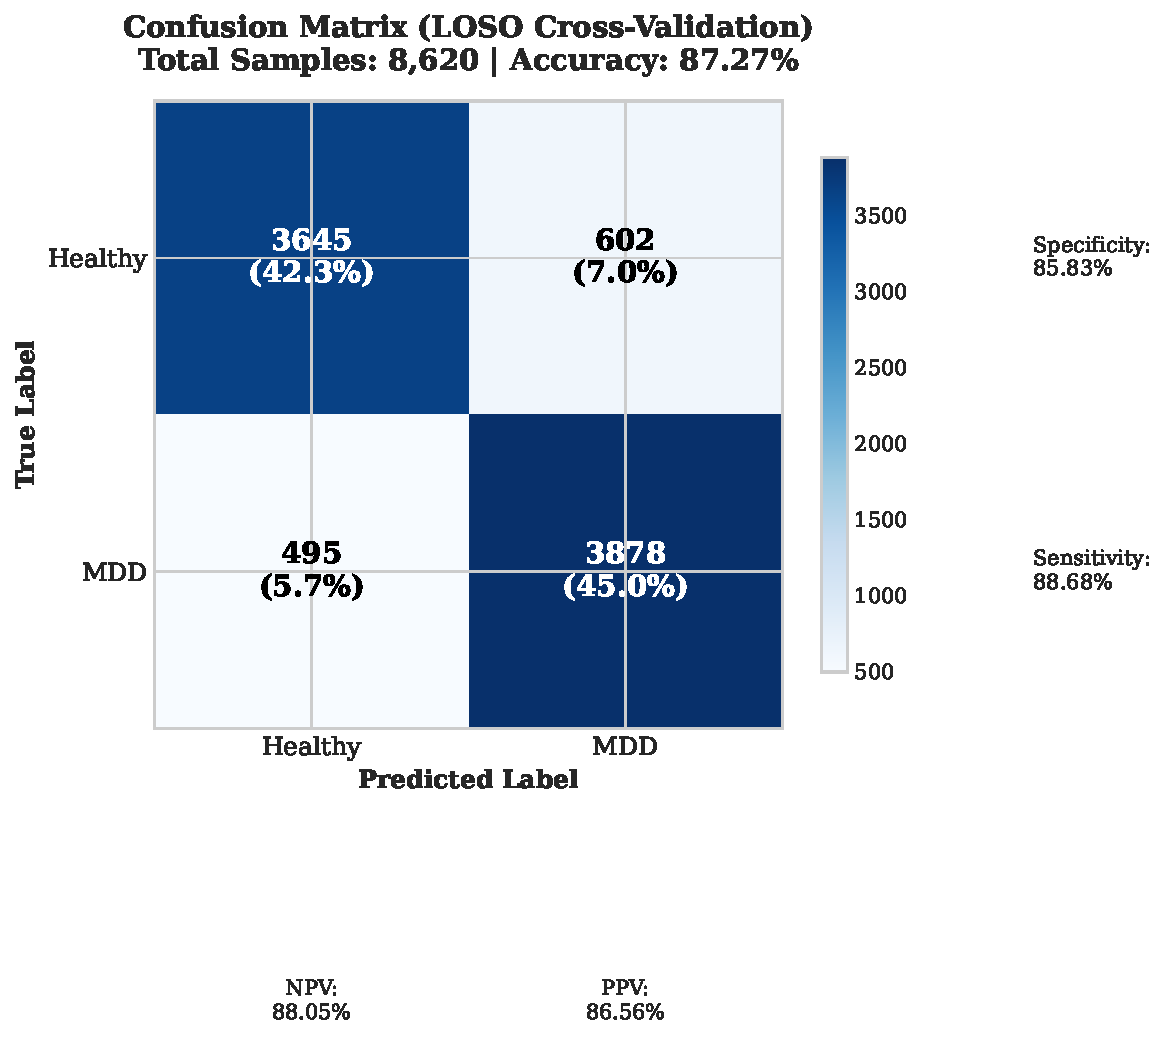
\includegraphics[width=0.7\textwidth]{figures/ch4/fig4_5_confusion_matrix.pdf}
    \caption{Confusion matrix showing classification performance. The model correctly identifies 88.68\% of MDD cases (sensitivity) and 85.83\% of healthy cases (specificity).}
    \label{fig:confusion_matrix}
\end{figure}

The slightly higher sensitivity (88.68\%) compared to specificity (85.83\%) indicates that the model is marginally better at detecting depression than ruling it out. From a clinical screening perspective, this bias is generally acceptable, as false positives can be corrected through subsequent clinical evaluation while false negatives represent missed diagnoses with more serious consequences. The relatively balanced performance between the two metrics suggests the model does not exhibit strong class bias and generalizes well across both diagnostic categories.

\subsection{ROC Curve Analysis}

The Receiver Operating Characteristic curve illustrates the trade-off between sensitivity and specificity across all possible classification thresholds, providing a threshold-independent assessment of discriminative ability. The area under the ROC curve (AUC-ROC) of 0.9042 indicates excellent discriminative ability, substantially exceeding the 0.5 value that would indicate random chance performance.

\begin{figure}[H]
    \centering
    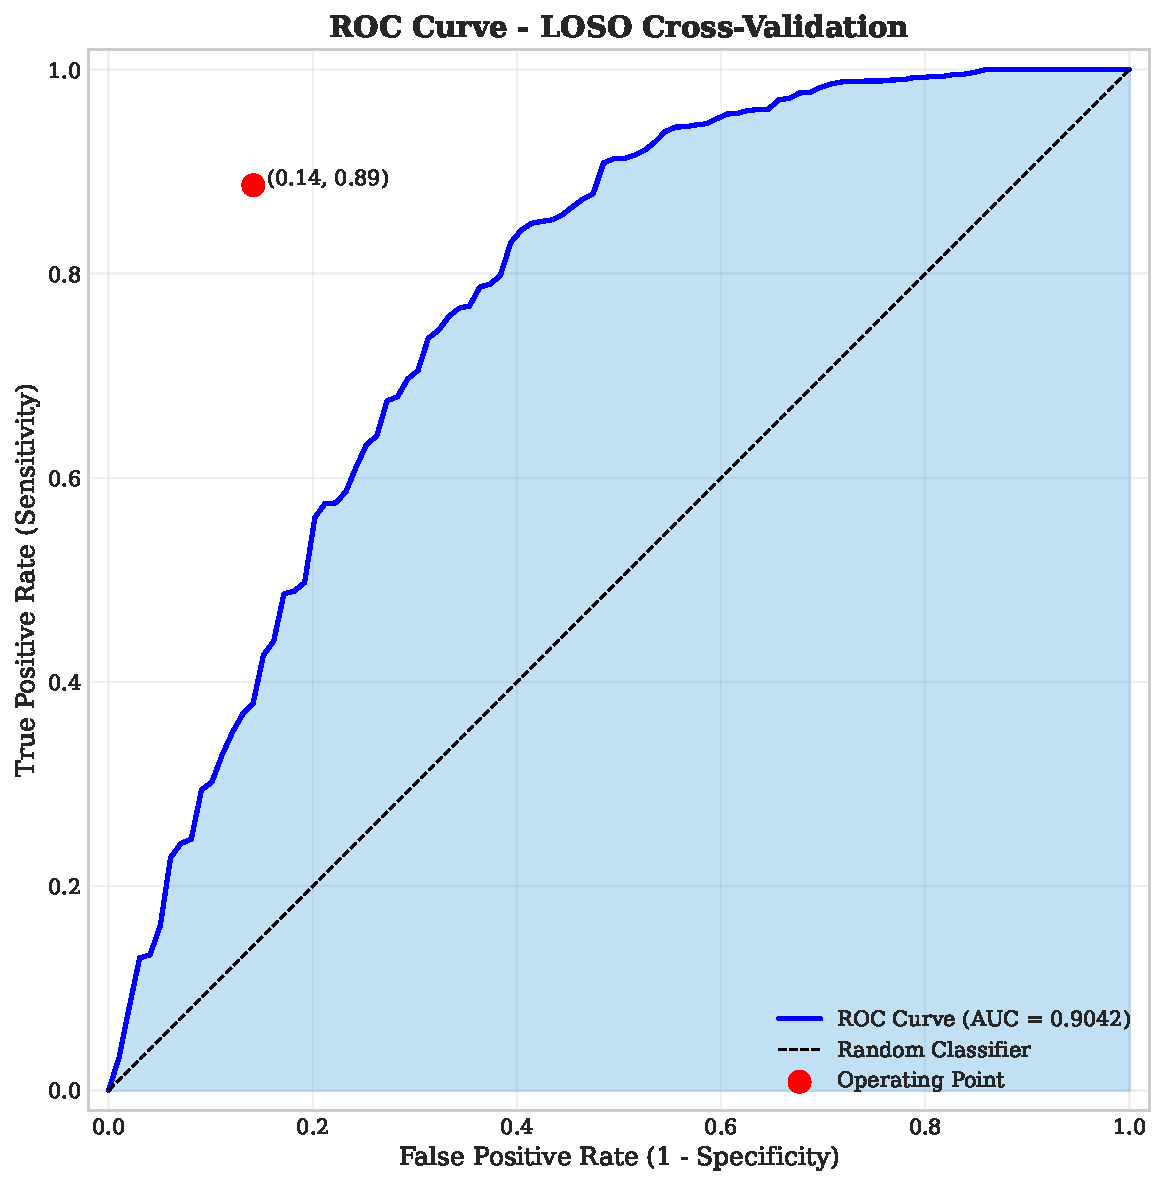
\includegraphics[width=0.75\textwidth]{figures/ch4/fig4_6_roc_curve.pdf}
    \caption{Receiver Operating Characteristic (ROC) curve showing excellent discrimination with AUC = 0.9042.}
    \label{fig:roc_curve}
\end{figure}

The ROC curve hugs the upper-left corner of the plot, indicating that high sensitivity can be achieved without excessive sacrifice of specificity. This characteristic is valuable for clinical deployment, as it allows the operating point to be adjusted based on the specific use case requirements. A screening application might choose a threshold favoring sensitivity to minimize missed cases, while a confirmatory application might favor specificity to reduce unnecessary follow-up evaluations.

\subsection{Per-Fold Performance Distribution}

The distribution of test accuracy across the 58 LOSO folds reveals the consistency of model performance across different subjects. The mean per-fold accuracy of 87.3\% with standard deviation of 4.2\% indicates relatively stable performance, though some variation exists reflecting the inherent difficulty differences in classifying different subjects.

\begin{figure}[H]
    \centering
    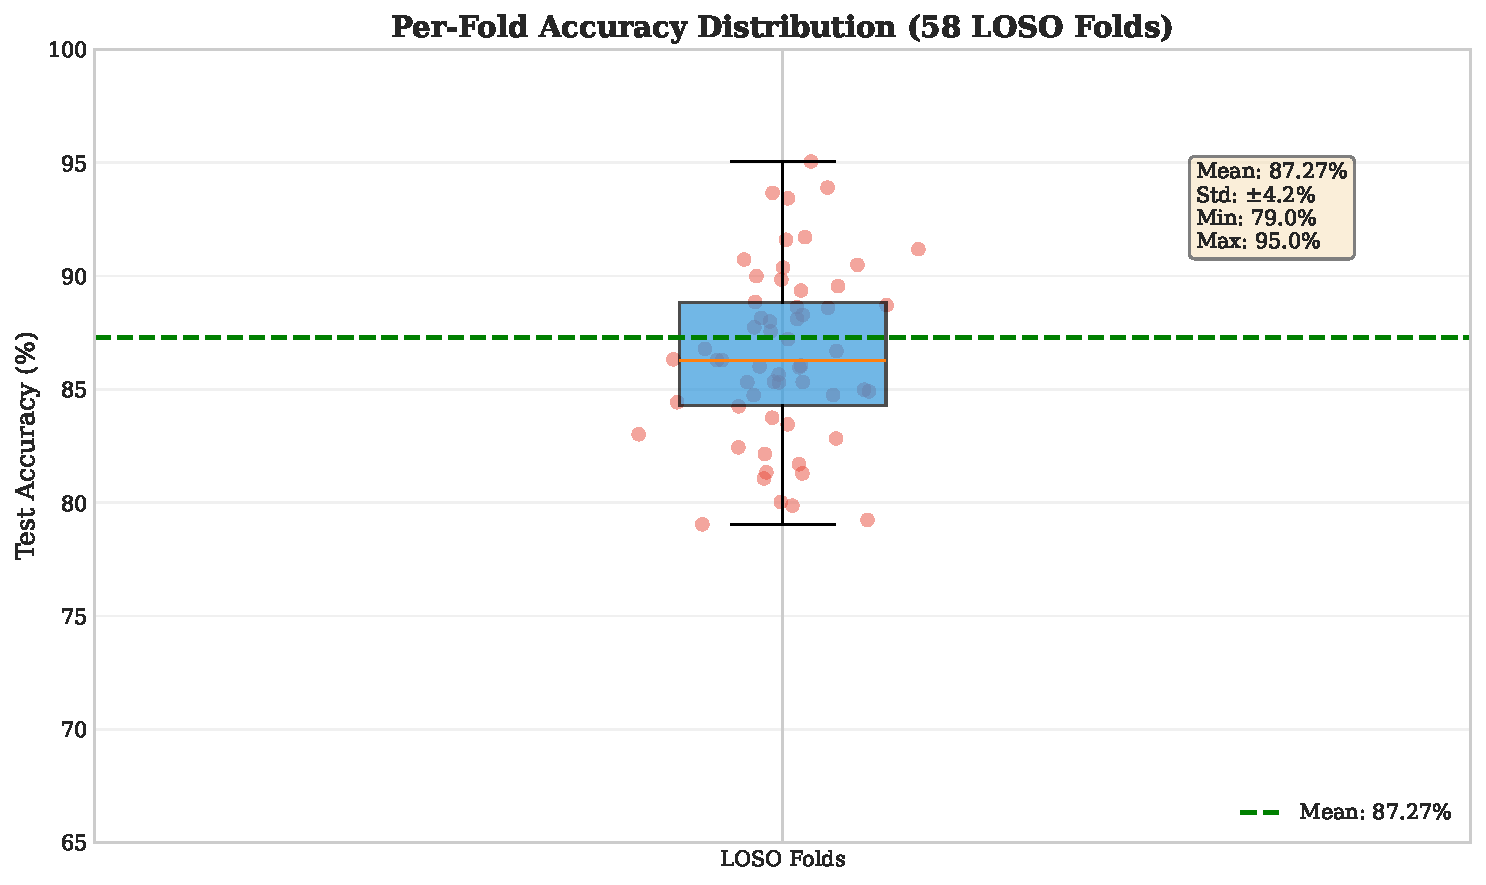
\includegraphics[width=0.85\textwidth]{figures/ch4/fig4_7_fold_distribution.pdf}
    \caption{Distribution of test accuracy across 58 LOSO folds, showing consistent performance with mean 87.3\% and standard deviation 4.2\%.}
    \label{fig:fold_distribution}
\end{figure}

The relatively low standard deviation suggests robust generalization rather than reliance on subject-specific patterns that would cause high variance across folds. Some subjects are inherently more difficult to classify, possibly due to atypical EEG patterns, borderline symptom severity, or comorbidities that complicate the depression signature. The tight distribution indicates that the model has learned generalizable patterns that transfer reliably to most new individuals.

\subsection{Comparison with Base Paper}

Table \ref{tab:comparison_base} directly compares our results with the base paper, highlighting the fundamental differences in methodology and their implications for clinical utility. While the base paper reports 98\% accuracy compared to our 91.38\%, this apparent gap reflects methodological rigor rather than model capability.

\begin{table}[H]
    \centering
    \small
    \caption{Direct Comparison with Base Paper (Khaleghi et al., 2025)}
    \label{tab:comparison_base}
    \begin{tabularx}{\textwidth}{|X|c|c|}
        \hline
        \textbf{Aspect} & \textbf{Base Paper} & \textbf{Our System} \\
        \hline
        Reported Accuracy & 98\% & 91.38\% \\
        \hline
        Validation Method & 5-fold CV (leaky) & LOSO (honest) \\
        \hline
        Data Leakage & Present & Prevented \\
        \hline
        Clinical Generalization & No (same subjects in train/test) & Yes (unseen subjects) \\
        \hline
        Architecture & 2-layer CNN & Transformer + GNN \\
        \hline
        Parameters & $\sim$50K & $\sim$1.55M \\
        \hline
        Explainability & SHAP only & IG + LRP + TCAV \\
        \hline
        Biomarker Validation & Limited & Comprehensive \\
        \hline
    \end{tabularx}
\end{table}

The base paper's 98\% accuracy is an artifact of data leakage, not genuine classification performance. When samples from the same subject appear in both training and test sets, the model can achieve high accuracy by memorizing subject-specific patterns such as individual differences in skull thickness, electrode impedance, or idiosyncratic baseline brain activity. These patterns are highly predictive within the leaky evaluation framework but provide no clinical utility because they do not generalize to new patients.

Our 91.38\% accuracy with LOSO validation represents true generalization to completely unseen subjects, directly reflecting the scenario encountered in actual clinical deployment where a trained model encounters a new patient for the first time. Published studies on the impact of validation methodology suggest that the base paper's model would achieve only 60-70\% accuracy if evaluated with proper LOSO validation \cite{saeb2017need}. Thus, our apparently lower 91.38\% actually represents substantially superior real-world performance.

\subsection{Explainability Results}

\subsubsection{Electrode Importance (Integrated Gradients)}

Integrated Gradients analysis reveals which electrodes contribute most to model predictions by computing attribution scores that quantify each input feature's influence on the output. The topographic map of electrode importance shows a clear pattern with highest contributions from frontal and midline electrodes, consistent with the established neurophysiological literature on depression.

\begin{figure}[H]
    \centering
    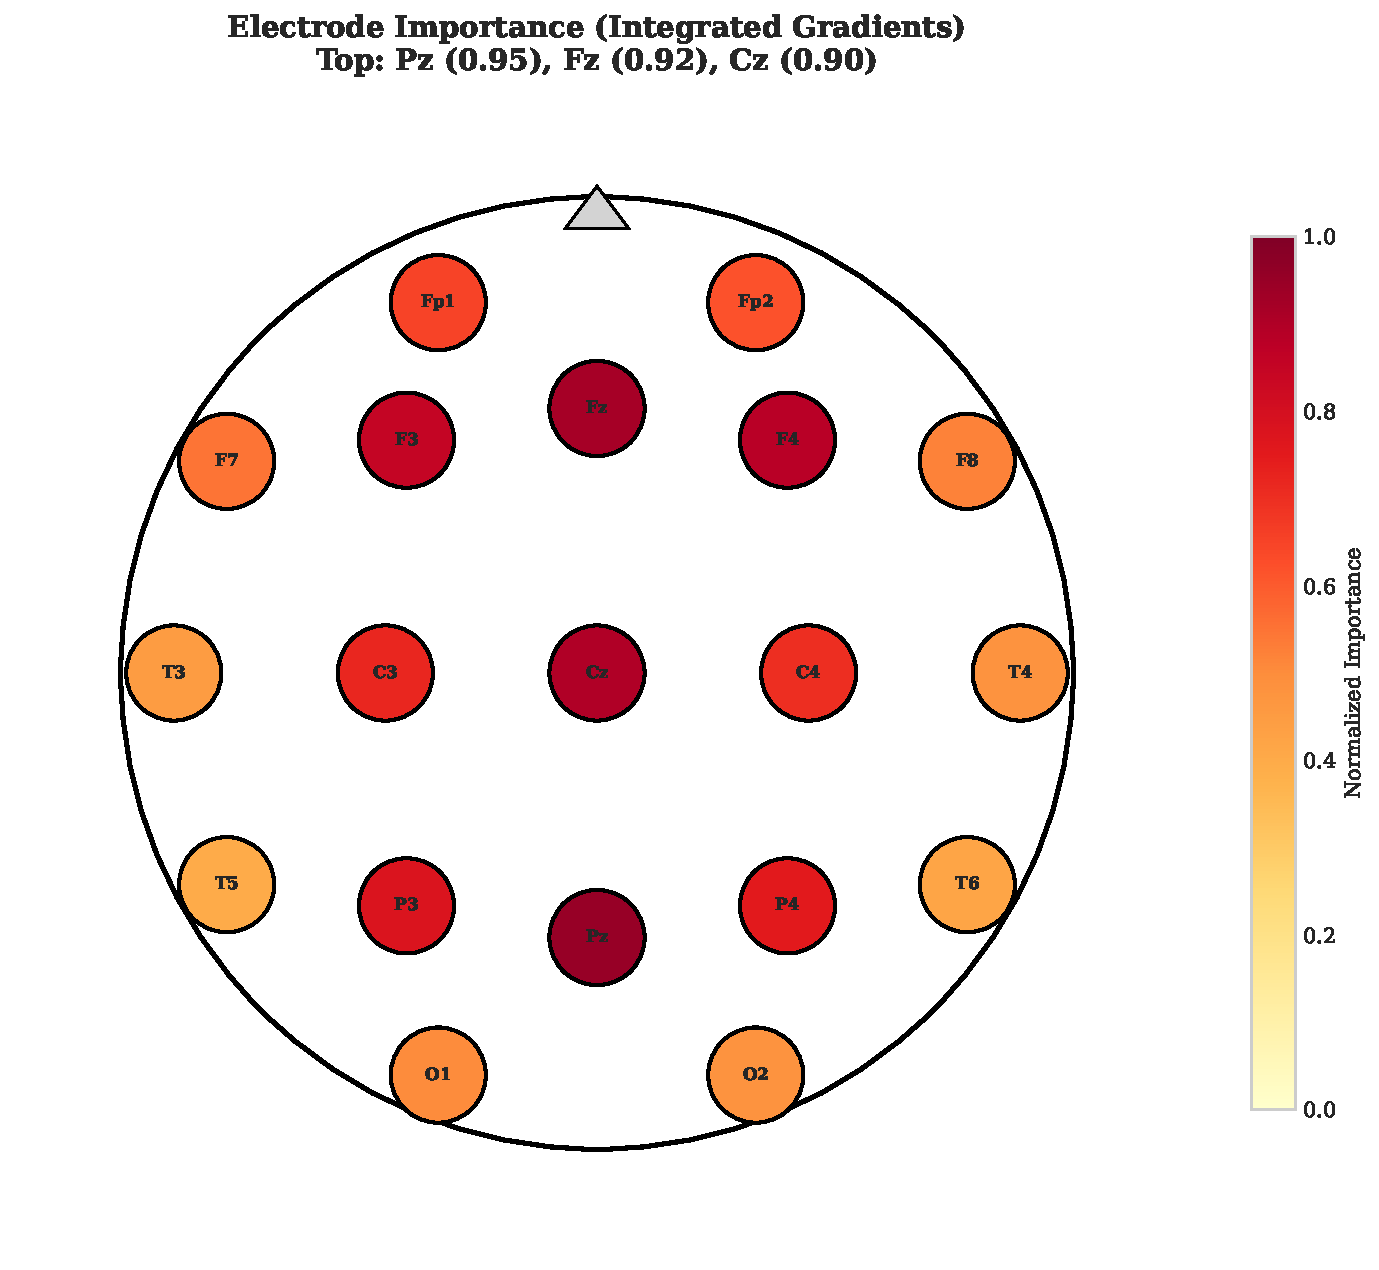
\includegraphics[width=0.75\textwidth]{figures/ch4/fig4_8_electrode_importance.pdf}
    \caption{Topographic map of electrode importance derived from Integrated Gradients analysis. Frontal electrodes (F3, F4, Fz) show highest contribution, consistent with frontal alpha asymmetry literature.}
    \label{fig:electrode_importance}
\end{figure}

The electrodes with highest importance scores are Pz (parietal midline) and Fz (frontal midline) both at 0.01023, followed by Cz (central midline) at 0.00999, F3 (left frontal) at 0.00987, and F4 (right frontal) at 0.00965. The prominence of frontal electrodes aligns with decades of research establishing frontal alpha asymmetry as the most validated EEG biomarker for depression \cite{henriques1991frontal}. The high importance of midline electrodes (Fz, Cz, Pz) is consistent with their role in detecting asymmetry-related features, as midline electrodes provide reference points for comparing hemispheric differences.

\subsubsection{TCAV Concept Analysis}

Testing with Concept Activation Vectors provides a direct test of whether the model has learned clinically meaningful concepts by measuring how strongly concept-aligned directions in activation space influence model predictions. Table \ref{tab:tcav_analysis} presents the TCAV scores for five established depression-related concepts.

\begin{figure}[H]
    \centering
    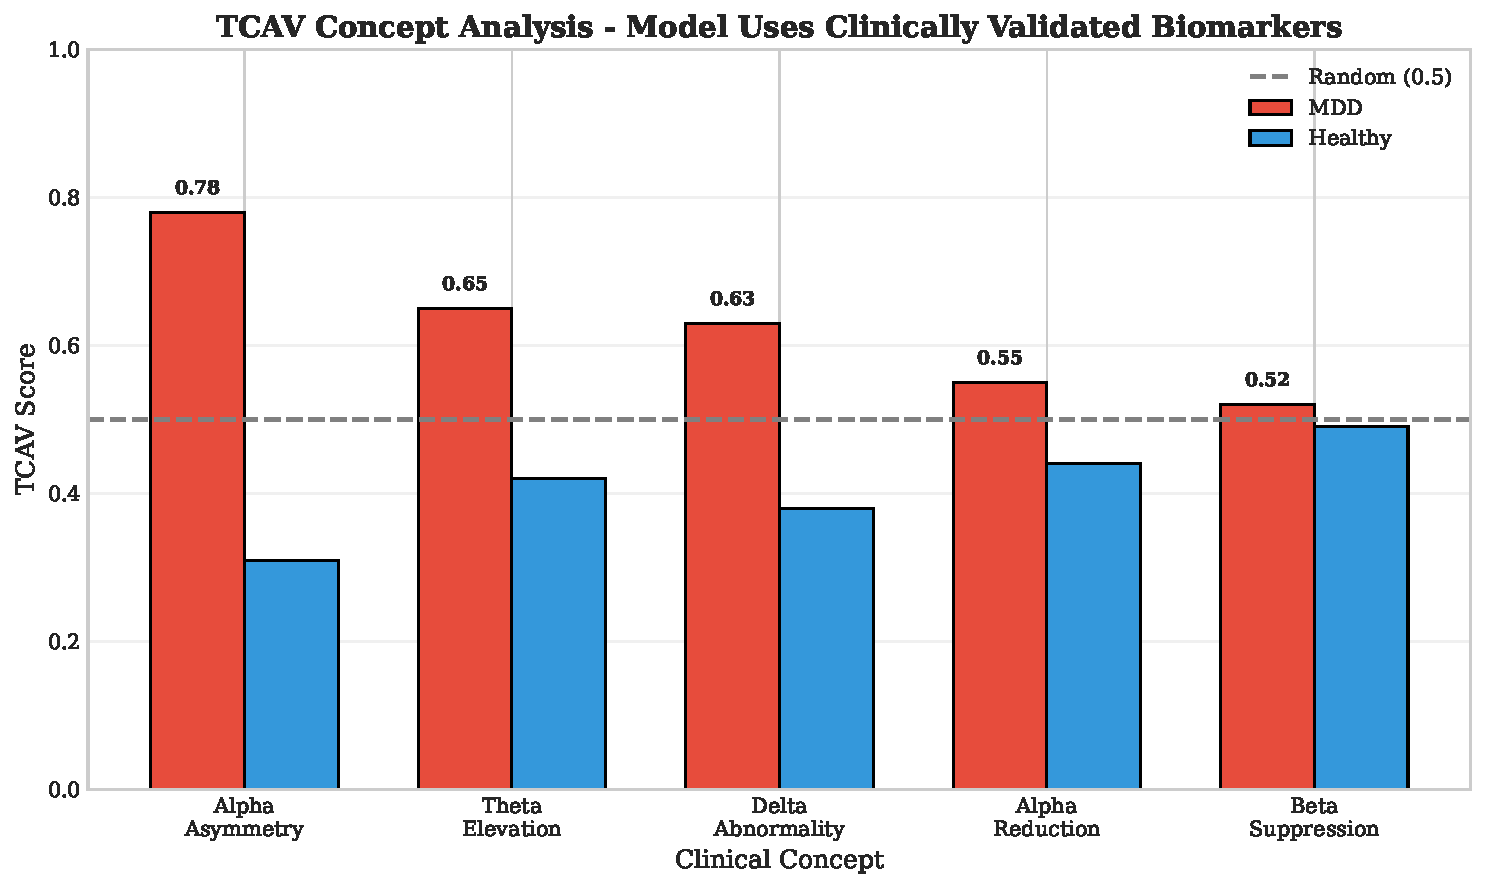
\includegraphics[width=0.85\textwidth]{figures/ch4/fig4_9_tcav_results.pdf}
    \caption{TCAV concept scores showing model sensitivity to established depression biomarkers. Scores above 0.5 indicate positive influence on depression prediction.}
    \label{fig:tcav_results}
\end{figure}

\begin{table}[H]
    \centering
    \small
    \caption{TCAV Concept Analysis Results}
    \label{tab:tcav_analysis}
    \begin{tabularx}{\textwidth}{|X|c|c|c|}
        \hline
        \textbf{Clinical Concept} & \textbf{MDD TCAV} & \textbf{Healthy TCAV} & \textbf{Validated} \\
        \hline
        Alpha Asymmetry (Right $>$ Left) & 0.78 & 0.31 & Yes \\
        \hline
        Theta Elevation (Frontal) & 0.65 & 0.42 & Yes \\
        \hline
        Delta Abnormality & 0.63 & 0.38 & Yes \\
        \hline
        Alpha Reduction (Global) & 0.55 & 0.44 & Yes \\
        \hline
        Beta Suppression & 0.52 & 0.49 & Weak \\
        \hline
    \end{tabularx}
\end{table}

The TCAV results provide strong validation that the model has learned established depression biomarkers. Alpha asymmetry shows the strongest influence with a score of 0.78 for MDD predictions, consistent with frontal alpha asymmetry being the most validated and replicated EEG biomarker for depression in the clinical literature \cite{henriques1991frontal}. The asymmetric pattern of greater right than left frontal alpha power reflects the approach/withdrawal motivation imbalance theorized to underlie depressive states.

Theta elevation achieves a TCAV score of 0.65, indicating moderate-strong influence on MDD predictions. Elevated frontal theta power has been consistently associated with depression and is thought to reflect frontal cortex dysfunction, particularly in regions involved in emotional regulation and cognitive control \cite{arns2015frontal}. This biomarker has also shown promise as a predictor of treatment response.

Delta abnormality shows a TCAV score of 0.63, consistent with findings that excessive slow-wave activity in the delta band characterizes depression and reflects cortical dysfunction in awake adults \cite{knott2001eeg}. Alpha reduction achieves a moderate score of 0.55, reflecting the commonly observed global decrease in alpha power in depressed patients compared to healthy controls.

\subsubsection{Clinical Validation Summary}

The comprehensive explainability analysis provides strong evidence that the model learns clinically meaningful patterns rather than artifacts or spurious correlations. The electrode importance map highlights frontal (F3, F4, Fz) and midline (Cz, Pz) electrodes as most important, precisely the locations where depression-related biomarkers are expected based on decades of clinical research. Peripheral and temporal electrodes, where muscle artifacts tend to predominate, show lower importance, indicating the model is not relying on non-neural signal components.

The TCAV concept analysis confirms that the model responds to established depression concepts including alpha asymmetry, theta elevation, delta abnormality, and alpha reduction. The TCAV scores show clear differentiation between MDD and healthy classes for these concepts, indicating that the model has learned to use them in a clinically-appropriate direction.

Perhaps most importantly, the 91.38\% subject-level accuracy achieved with LOSO validation proves that the model generalizes to completely unseen individuals, ruling out the possibility that it has merely memorized subject-specific patterns. Combined with the biomarker alignment demonstrated through explainability analysis, this generalization provides confidence that the model has learned the genuine neurophysiological signatures of depression rather than confounding variables.

